\chapter{Methods}
\label{sec:methods}

\section{Learning a flexible joint posterior with a generalized $f$-Mean}
As introduced herein, we are working with a multi modal VAE (mmVAE), which learns a joint distribution that contains the combined information of each learned uni modal latent distribution.
For $M$ modalities, $M$ different encoder and decoder pairs are needed, each encoder learning a unimodal latent distribution $\unimodalpost$.
To learn a joint distribution of multiple data modalities, some function $\mathcal{F}$ is needed that merges the information from all unimodal latent distributions into one joint distribution (see \cref{fig:magic_graph}).
In previous work \parencite{poe,shi_variational_2019,sutter_generalized_2020}, learning a joint distribution has been done effectively by combining learned unimodal distributions with a PoE \parencite{poe}, an MoE \parencite{shi_variational_2019} or both \parencite{sutter_generalized_2020}.
While for both the MoE and PoE, reasons have been established why they are good choices for the aggregation function, both come with several shortcomings (\cref{subsec:Multi Modal VAEs}).
A more flexible and generic function could improve the fusion of information from each modality and improve the expressiveness of the joint posterior.

To this end, we generalize previous methods and implement the fusion of the uni modal latent distributions utilizing a trainable generalized $f$-mean, with parameters $\psi$.

Since the generalized $f$-Mean is a generalisation of the arithmetic and the geometric mean, it should bring results that are at least equally good or better than previous results if the objective is right.
E.g. if the geometric or the arithmetic mean were the best functions to merge the uni modal posteriors, the model could learn parameters $\psi$ such that the $f$-Mean equals an arithmetic or geometric mean.

The generalized $f$-Mean is defined as follows:
\begin{equation}
    \label{gfm}
    \mathcal{M}_{f}\left( \textbf{p} \right) = f^{-1}\left( \frac{1}{N} \sum ^N _{i=1} f(\textbf{p}_i)) \right)
\end{equation}

In \cref{gfm}, $f$ can be anything as long as it is invertible and differentiable.
Normalizing Flows \parencite{papamakarios_normalizing_2019} present an approach to implement a sequence of invertible transformations with neural networks and provide a natural implementation for a parameterized $f_{\psi}$.
We refer to \cref{subsec: Normalizing Flows} for a more in-depth introduction to normalizing flows.





\begin{figure}[h!]
    \centering
    \resizebox{\textwidth}{!}{%
        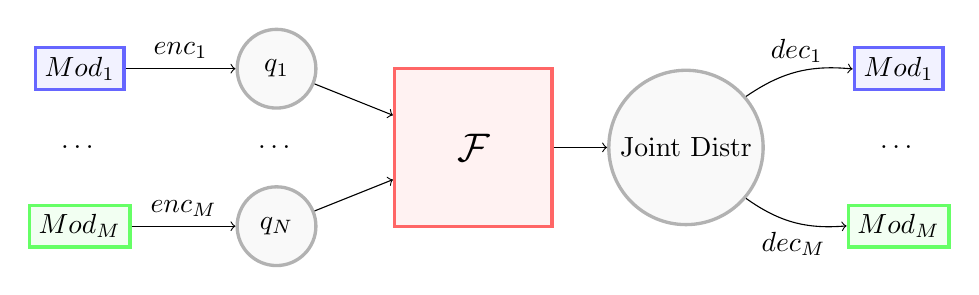
\begin{tikzpicture}[Mod1/.style={rectangle, draw=blue!60, fill=blue!5, very thick, minimum size=5mm},Mod2/.style={rectangle, draw=green!60, fill=green!5, very thick, minimum size=5mm},enc_mods/.style={circle, draw=gray!60, fill=gray!5, very thick, minimum size=10mm},magic/.style={rectangle, draw=red!60, fill=red!5, very thick, minimum size=20mm},]
            \node[Mod1] (mod1) {$Mod_1$};
            \node[below of=mod1] (points) {\ldots};
            \node[enc_mods, right of=mod1, xshift=1.5cm] (q1) {$q_1$};
            \node[Mod2, below of=points] (modn) {$Mod_M$};
            \node[enc_mods, right of=modn, xshift=1.5cm] (q2) {$q_N$};
            \node[below of=q1] (points) {\ldots};
            \node[magic, right of=q1, yshift=-1cm, xshift=1.5cm] (magic) {\Large$\mathcal{F}$};
            \node[enc_mods, right of=magic, xshift=1.7cm] (joint) {Joint Distr};
            \node[Mod1, right of=joint, xshift=1.7cm,yshift=+1cm] (rec_mod1) {$Mod_1$};
            \node[right of=joint,xshift=1.7cm] (points) {\ldots};
            \node[Mod2, right of=joint, xshift=1.7cm,yshift=-1cm] (rec_mod2) {$Mod_M$};
            \draw[->] (mod1) -- node[anchor=south] {$enc_1$} (q1);
            \draw[->] (q1) -- (magic);
            \draw[->] (modn) -- node[anchor=south] {$enc_M$} (q2);
            \draw[->] (q2) -- (magic);
            \draw[->] (magic) -- (joint);
            \draw[->] (joint) edge[bend left=20] node[anchor=south] {$dec_1$} (rec_mod1);
            \draw[->] (joint) edge[bend right=20] node[anchor=north] {$dec_M$} (rec_mod2);
        \end{tikzpicture}
    }
    \caption{\textbf{Flowchart depicting the main elements of a multi modal VAE wit $M$ different modalities.}
    Each input modality $m$ gets mapped to a unimodal latent distribution $q_m$ by an encoder $enc_m$.
    The $M$ unimodal learned distributions then get merged by a function $\mathcal{F}$ into a joint distribution from which the decoders can sample in order to reconstruct each of the $M$ modalities.}
    \label{fig:magic_graph}
\end{figure}

%%%%%%%%%%%%%%%%%%%%%%%%%%%%%%%%%%%%%%%%%%%%%%%%%%%%%%%%%%%%%%%%%%%%%%%%%%%%%%%%%%%%%%%%%%%%%%%%%%%%%%%%%%%%%%%%%%%%%%%%%%%%%%%%%%%%%%%%%%%%%%%%%%%%%%%%%%%%%%%%%%%%%%%%%%%%%%%%%%%%%%%%%%%%%%%%%%%%

\section{Evaluating the joint posterior distribution}
The main difficulty in our approach comes from the fact that the $f$-mean of the uni modal approximations follows an unknown distribution.
While this makes the joint distribution more flexible, this also makes the computation of the regularization term in the ELBO, the KL-divergence, more difficult to compute.
In fact, if the density of the joint distribution is unknown, it is impossible to compute the KL-divergence in closed form.

An intuitive alternative would be to find an upper bound of the KL-divergence which can be computed in closed from, such that it can be minimized in order to minimize the true divergence:
\begin{equation}
    \label{eq:kldivbound}
    \begin{split}
    D_{KL}^{\prime} &\geq D_{KL}(\mathcal{M}_f(\{\unimodalpost\ \forall\ \xsetm \in \xsubset\}))\\
    &=  D_{KL}\left(f^{-1}\left(\sum _{\xsetm \in \xsubset} \frac{f(\unimodalpost)}{|\xsubset|}\right)\ ||\ \prior\right)
    \end{split}
\end{equation}

Using the change of variable formula (\cref{eq:changeofvariables}), the $f$-mean in \cref{eq:kldivbound} can be rewritten as follows:
\begin{equation}
    \mathcal{M}_f = f^{-1}(Q)|J_{f^{-1}}(Q)|
\end{equation}
with
\begin{equation}
    Q= \sum _{\xsetm \in \xsubset} \frac{\unimodalpost|J_f(\unimodalpost)|}{|\xsubset|}
\end{equation}

Here Q is a sum of random variables, which can be rewritten as chained convolutions \citep{sorv} and is hard to evaluate.

Instead, we propose four workarounds to the computation of the KL-divergence in \cref{eq:kldivbound}.
\begin{enumerate}

    \item For one, \cref{eq:kldivbound} can be simplified by skipping the backwards transformation $f^{-1}$.
    This leads to a mixture of transformed posteriors, which divergence can be bounded using \cref{lemma:DklLowerBound} from \parencite{sutter_multimodal_2020}.

    We then get an upper bound that can be minimized:
    \begin{equation}
        \begin{split}
            &D_{KL}\left(\sum _{\xsetm \in \xsubset} \frac{f_{\psi}(\unimodalpost)}{|\xsubset|}\ ||\ \prior\right)\\
            &\leq \frac{1}{|\xsubset|} \sum  _{\xsetm \in \xsubset} D_{KL} \left(f_{\psi} (\unimodalpost))||\ \prior \right)
        \end{split}
    \end{equation}

    We implement this in the Mixture of flow of product of experts (\mg{MofoPoE}) model, which is described in \cref{subsec:mofopoe}.

    \item Another way to simplify the KL-divergence in \cref{eq:kldivbound} is to force the output of the $f$-mean to be a Gaussian distribution.
    This can be done by, instead of mixing the posteriors which follow a normal distribution, mixing their parameters $\mu_s$ and $\sigma_s$.
    The joint posterior is then described as follows:
    \begin{equation}
        \label{eq:qjointmopgfm}
        q_{\phi, joint} \sim \mathcal{N}\left(  f_{\mu}^{-1}(\sum _{\xsetm \in \xsubset} \frac{f_{\mu}(\mu_s)}{|\xsubset|}),\ f_{\sigma}^{-1}(\sum  _{\xsetm \in \xsubset} \frac{f_{\sigma}(\sigma_s^2)}{|\xsubset|})\right)
    \end{equation}

    This is implemented as the mixture of parameter generalized $f$-mean (\mg{MopgfM}) and described in \cref{subsec:mopgfm}.

    \item The sum of random variables in the $f$-mean (\cref{eq:kldivbound}) is hard to evaluate since the transformed uni modal posteriors ($\unimodalpost$) follow an unknown distribution.
    It is however possible to steer the normalizing flow $f_{\psi}$ to map $\unimodalpost$ towards a normal distribution, such that the sum of random variables can be evaluated.
    This normal distribution can be amortized by making it dependent on the input.
    We implement this as the \mg{MogfM\_amortized} method, described in \cref{subsubsec:mogfm_amortized}.

    \item Instead of evaluating the density of the sum of random variables inside the $f$-mean, we investigate if it is possible to approximate it with a normal distribution.
    The mean and variance can be inferred using importance samples from the sum of random variables.
    We implement this as the importance weighted mixture of generalized $f$-mean (\mg{iwMogfM}), described in \cref{subsubsec:iwMogfM}.

\end{enumerate}

%%%%%%%%%%%%%%%%%%%%%%%%%%%%%%%%%%%%%%%%%%%%%%%%%%%%%%%%%%%%%%%%%%%%%%%%%%%%%%%%%%%%%%%%%%%%%%%%%%%%%%%%%%%%%%%%%%%%%%%%%%%%%%%%%%%%%%%%%%%%%%%%%%%%%%%%%%%%%%%%%%%%%%%%%%%%%%%%%%%%%%%%%%%%%%%%%%%%

\section{Models}
In this section, we describe the models that implement the four methods introduced above and enumerate their advantages and disadvantages.

%%%%%%%%%%%%%%%%%%%%%%%%%%%%%%%%%%%%%%%%%%%%%%%%%%%%%%%%%%%%%%%%%%%%%%%%%%%%%%%%%%%%%%%%%%%%%%%%%%%%%%%%%%%%%%%%%%%%%%%%%%%%%%%%%%%%%%%%%%%%%%%%%%%%%%%%%%%%%%%%%%%%%%%%%%%%%%%%%%%%%%%%%%%%%%%%%%%%

\subsection{Mixture of flow of Products of Experts}\label{subsec:mofopoe}
The Mixture of flow of Products of Experts (\mg{MofoP}) builds on the \mg{MoPoE} by transforming the subset posterior approximations $\subsetpost$ with a series of F invertible transformations with trainable parameters $\psi$:
\begin{equation}
    z_{F,S} =f_{\psi}(z_{0,S} \sim \subsetpost) = f_F \circ \ldots \circ f_2 \circ f_1(z_{0,S} \sim \subsetpost)
\end{equation}

The density of the resulting transformed subset posterior distribution can be evaluated with the change of variables formula (\cref{eq:changeofvariables}):
\begin{equation}
    \label{eq:changeofvariables_}
    \ln f(\subsetpost) = \ln q_\phi (z_0|\xsubset) - \sum _{i=1} ^{F}\ln \left|  \det \frac{df_i}{dz_{i-1}}\right|
\end{equation}

Here $f(\subsetpost)$ can follow any distribution and is thus more flexible than the gaussian subset posterior approximation in the \mg{MoPoE} model.
A flow chart depiction of the \mg{MofoP} is shown in \cref{fig:mofopoe}.
During a forward pass, a sample is taken from each subset posterior distribution, transformed with a normalizing flow $f$ and then mixed with a MoE.

The resulting objective can be written as follows, by slightly modifying the \mg{MoPoE} objective from \cref{eq:mopoe_}:

\begin{equation}
    \begin{split}
        &\mathcal{L}_{\mg{MofoP}}(\theta, \phi, \psi; \xset)\\
        &=  \mathbb{E}_{q_{\phi}(\textbf{z}|\mathbb{X})}[\log (p_{\theta}(\mathbb{X}|\textbf{z}))] - \frac{1}{2^M} \sum _{\mathbb{X}_s \in \mathcal{P}(\mathbb{X})} D_{KL}\biggl( \tilde{q}_{\phi}(\textbf{z}|\mathbb{X}_s)\ ||\ p_{\theta}(\textbf{z})\biggr)\\
        &= \mathbb{E}_{q_{\phi}(\textbf{z}|\mathbb{X})}[\log (p_{\theta}(\mathbb{X}|\textbf{z}))] - \frac{1}{2^M} \sum _{\mathbb{X}_s \in \mathcal{P}(\mathbb{X})} D_{KL}\biggl( f_{\psi} (\unimodalpost))\ ||\ p_{\theta}(\textbf{z})\biggr)
    \end{split}
\end{equation}

The KL-divergence between the transformed subset posteriors and the prior can be evaluated as follows using \cref{eq:changeofvariables_}:

\begin{equation}
    \begin{split}
        &D_{KL}\biggl( f_{\psi} (\unimodalpost))\ ||\ p_{\theta}(\textbf{z})\biggr)\\
        &= \mathbb{E}_{f_{\psi}(q_{\phi_m})} \left[ \log  f_{\psi} (q_{\phi_m}(f_{\psi}(z)|x_m)) - \log p_{\theta}(f_{\psi}(z))   \right]\\
        &= \mathbb{E}_{q_{\phi_m}} \left[ \log  q_{\phi_m}(z|x_m) - \log \det J_{f_{\psi}} - \log p_{\theta}(f_{\psi}(z))   \right]\\
    \end{split}
\end{equation}

We use the \mg{MofoP} method in comparison to the other methods that make use of the inverse transform $f^{-1}$ to evaluate if the merging of information between unimodal posteriors can be improved by simply making the subsets more flexible. % todo

One advantage of the \mg{MofoP} method is that since the inverse of the flow transformation is not needed, implementations of normalizing flows can be used where the evaluation of the inverse flow does not need to be tractable.
This gives more flexibility in the choice of the flow implementation.

\begin{figure}[h!]
    \centering
    \resizebox{\textwidth}{!}{%
        \py{pytex_printonly(script='scripts_/mofop_graph.py', data = '')}
    }
    \caption{\textbf{Fowchart depicting the \mg{MofoP} method.} The \mg{MofoP} creates more expressive subset posteriors by transforming the PoE posteriors with a series of invertible transformations.
    Here, an example with 2 subsets is shown. On the left side are the two input modalities from the polymnist dataset (see \cref{polymnist}), on the right side are the generated samples.
    In the header of each generated sample is described from which subset the decoder sampled for the generation (left side of the $\rightarrow$) and which modality was generated (right side of the $\rightarrow$).}
    \label{fig:mofopoe}
\end{figure}

%%%%%%%%%%%%%%%%%%%%%%%%%%%%%%%%%%%%%%%%%%%%%%%%%%%%%%%%%%%%%%%%%%%%%%%%%%%%%%%%%%%%%%%%%%%%%%%%%%%%%%%%%%%%%%%%%%%%%%%%%%%%%%%%%%%%%%%%%%%%%%%%%%%%%%%%%%%%%%%%%%%%%%%%%%%%%%%%%%%%%%%%%%%%%%%%%%%%

\subsection{Mixture of parameter generalized $f$-means}\label{subsec:mopgfm}
% the main disadvantage here is that this method requires many parameters (needs two flows) but has not much flexibility
The Mixture of parameter generalized $f$-mean (\mg{Mopgfm}) mixes the means and the standard deviations of the unimodal posteriors, in order to obtain a normal distribution that depends on each of the uni modal posteriors (see \cref{eq:qjointmopgfm}).
The aggregation over the means and the standard deviations is done with a parameterized $f$-mean.

\smallskip

This is a generalisation of the PoE method since a product of gaussian experts is itself Gaussian with mean $\mu_{PoE} = (\sum _i \mu _i V_i)(\sum _i V_i)^{-1}$ and covariance $V_{PoE}= (\sum _i V_i)^{-1}$ where $\mu _i, V_i$ are the parameters of the $i$-th Gaussian.\\
Without loss of generality, it can be assumed that:\\
$f_{\mu}^{-1}(\sum _{\xsetm \in \xsubset} \frac{f_{\mu}(\mu_s)}{|\xsubset|}) = \mu_{PoE}$\quad and\quad $f_{\sigma}^{-1}(\sum  _{\xsetm \in \xsubset} \frac{f_{\sigma}(\sigma_s^2)}{|\xsubset|}) = V_{PoE}$.

\smallskip

The main advantage of this method is that since it is a generalisation of the PoE, it gives more flexibility to the modality fusion.
However, this comes at the cost that the expressiveness of the joint distribution is limited by being a Gaussian, and since the transformations are applied on the parameters of the uni modal distributions, transparency of the resulting transformation is lost.
It is hard, if not impossible, to translate \cref{eq:qjointmopgfm} into the following equation:
\begin{equation}
    q_{\phi, joint} = T(\{\unimodalpost \forall \xsetm \in \xset\})
\end{equation}
with T a well defined transformation.
The internal workings of the \mg{MopgfM} method are depicted in a simplified manner in \cref{fig:mopgfm}.


\begin{figure}[h!]
    \centering
    \resizebox{\textwidth}{!}{%
        \py{pytex_printonly(script='scripts_/mopgfm_graph.py', data = '')}
    }
    \caption{\textbf{The \mg{MopgfM} makes use of the $f$-mean to aggregate the means und standard deviations of the unimodal posteriors create $2^M$ normally distributed subsets, which are then merged with a MoE.} Here, an example with 2 subsets is shown. On the left side are the two input modalities from the polymnist dataset (see \cref{polymnist}), on the right side are the generated samples.
    In the header of each generated sample is described from which subset the decoder sampled for the generation (left side of the $\rightarrow$) and which modality was generated (right side of the $\rightarrow$).}
    \label{fig:mopgfm}
\end{figure}

%%%%%%%%%%%%%%%%%%%%%%%%%%%%%%%%%%%%%%%%%%%%%%%%%%%%%%%%%%%%%%%%%%%%%%%%%%%%%%%%%%%%%%%%%%%%%%%%%%%%%%%%%%%%%%%%%%%%%%%%%%%%%%%%%%%%%%%%%%%%%%%%%%%%%%%%%%%%%%%%%%%%%%%%%%%%%%%%%%%%%%%%%%%%%%%%%%%%


\subsection{Amortized Mixture of generalized $f$-means}\label{subsubsec:mogfm_amortized}
For the Amortized Mixture of generalized $f$-means (\mg{MogfM\_amortized}) method, we introduce a new loss $\mathcal{L}_2$ that pushes $f_{\psi}$ to map the uni modal posteriors to an amortized prior distribution, i.e. such that:

\begin{equation}
    \label{eq:amortizedprior}
    f_{\psi}(\unimodalpost) \sim \mathcal{N}(f_{\psi}(\mu_m), \textbf{I})
\end{equation}

Then, the density of the sum of random variables $\textbf{G}_f$ can easily be evaluated with:
\begin{equation}
    \textbf{G}_f(\textbf{z}|\textbf{x}_{1:|\xsubset|}) =\sum _{\xsetm \in \xsubset} \frac{f(\unimodalpost)}{|\xsubset|} \sim \mathcal{N} \left(  \sum _{m \in \xsubset} \frac{f(\mu_m)}{|\xsubset|}, \frac{1}{\sqrt{|\xsubset|}}  \cdot \textbf{I} \right)
\end{equation}

\Cref{eq:amortizedprior} can be achieved by minimizing the KL-divergence between the transformed uni modal posteriors and the amortized prior:
\begin{equation}
    \begin{split}
        \mathcal{L}_2 &= \sum _{\xsetm \in \xset} D_{KL}\left( f(\unimodalpost)\ ||\ \mathcal{N}(f(\mu_m), \textbf{I}) \right)\\
        &= \sum _{\xsetm \in \xset} D_{KL}\left( f(\unimodalpost)\ ||\ p_{\theta_m}(\textbf{z}) \right)\\
        &=  \sum _{\xsetm \in \xset} \mathbb{E}_{f(\unimodalpost)} [\log f(\unimodalpost) - \log p_{\theta_m}(\textbf{z})]\\
        &=  \sum _{\xsetm \in \xset} \mathbb{E}_{z_m \sim \unimodalpost} [\log q_{\phi_m}(z_m|\textbf{x}_M) - \log \det J_f  - \log p_{\theta_m}(f(z_m))]\\
    \end{split}
\end{equation}

The ELBO can then be evaluated as following:
\begin{equation}
    \begin{split}
        \mathcal{L}_1 &=  \mathbb{E}_{q_{\phi}(\textbf{z}|\mathbb{X})}[\log (p_{\theta}(\mathbb{X}|\textbf{z}))] -  \frac{1}{2^M} \sum _{\mathbb{X}_s \in \mathcal{P}(\mathbb{X})} D_{KL}\biggl( \tilde{q}_{\phi}(\textbf{z}|\mathbb{X}_s)\ ||\ p_{\theta}(\textbf{z})\biggr)\\
        &= \mathbb{E}_{q_{\phi}(\textbf{z}|\mathbb{X})}[\log (p_{\theta}(\mathbb{X}|\textbf{z}))] - \frac{1}{2^M} \sum _{\mathbb{X}_s \in \mathcal{P}(\mathbb{X})} \mathbb{E}_{\tilde{q}_{\phi}(\textbf{z}|\mathbb{X}_s)}[\log \tilde{q}_{\phi}(\textbf{z}|\mathbb{X}_s) - \log p_{\theta}(\textbf{z}) ]\\
        &= \mathbb{E}_{q_{\phi}(\textbf{z}|\mathbb{X})}[\log (p_{\theta}(\mathbb{X}|\textbf{z}))] - \frac{1}{2^M} \sum _{\mathbb{X}_s \in \mathcal{P}(\mathbb{X})} \mathbb{E}_{\textbf{G}_f(\textbf{z}|\textbf{x}_{1:|\xsubset|})}[\log \textbf{G}_f(\textbf{z}|\textbf{x}_{1:|\xsubset|})\\
        &\quad + \log \det J_{f^{-1}}- \log p_{\theta}(\textbf{z}) ]
    \end{split}
\end{equation}

The total loss is then:
\begin{equation}
    \begin{split}
        &\mathcal{L} = \mathcal{L}_1 + \mathcal{L}_2\\
        &= \mathbb{E}_{q_{\phi}(\textbf{z}|\mathbb{X})}[\log (p_{\theta}(\mathbb{X}|\textbf{z}))] - \frac{1}{2^M} \sum _{\mathbb{X}_s \in \mathcal{P}(\mathbb{X})} \mathbb{E}_{\textbf{G}_f(\textbf{z}|\textbf{x}_{1:|\xsubset|})}[\log \textbf{G}_f(\textbf{z}|\textbf{x}_{1:|\xsubset|})\\
        &\quad + \log \det J_{f^{-1}}- \log p_{\theta}(\textbf{z}) ]\\
        &\quad + \sum _{\xsetm \in \xset} \mathbb{E}_{z_m \sim \unimodalpost} [\log q_{\phi_m}(z_m|\textbf{x}_M) - \log \det J_f  - \log p_{\theta_m}(f(z_m))]
    \end{split}
\end{equation}

The resulting joint posterior $\textbf{G}_f$:
\begin{equation}
    \textbf{G}_f(\textbf{z}|\textbf{x}_{1:|\xsubset|}) =\sum _{\xsetm \in \xsubset} \frac{f(\unimodalpost)}{|\xsubset|}
\end{equation}
of the \mg{MogfM\_amortized} method can follow any distribution and can thus be more expressive than the joint posterior in the \mg{MopgfM} or \mg{MoPoE} methods.
The main disadvantage of this method is that the KL-divergence term in $\mathcal{L}_1$ can only be evaluated when the flow $f$ has already learned to map the uni modal posteriors towards the amortized priors.

%%%%%%%%%%%%%%%%%%%%%%%%%%%%%%%%%%%%%%%%%%%%%%%%%%%%%%%%%%%%%%%%%%%%%%%%%%%%%%%%%%%%%%%%%%%%%%%%%%%%%%%%%%%%%%%%%%%%%%%%%%%%%%%%%%%%%%%%%%%%%%%%%%%%%%%%%%%%%%%%%%%%%%%%%%%%%%%%%%%%%%%%%%%%%%%%%%%%


\subsection{Importance Weighted Mixture of generalized $f$-means} \label{subsubsec:iwMogfM}
The central limit theorem states that a sum of independent random variables tends towards a normal distribution, even if the original variables themselves are not normally distributed.
With the Importance Weighted Mixture of generalized $f$-means (\mg{iwMogfM}) method, we evaluate if the sum of unimodal posteriors from \cref{eq:kldivbound} can be approximated with a normal distribution.
It is important to note that since the unimodal posteriors should contain shared information they are assumed to be dependent such that the independence condition for the central limit theorem is not met.
We find however that the normal distribution with inferred parameters is a useful proxy which allows to evaluate the KL-divergence term in the objective from \cref{vaeelbo}.
To infer the parameters of the normal distribution, we take K importance samples from the sum of unimodal posteriors and evaluate their average and variance.
Importance sampling from the posterior has been done before for the \mg{iwVAE} in \cite{burda_importance_2016} (see \cref{subsec:iwvae}).

Like the \mg{MoPoE}, the \mg{iwMogfM} creates the joint posterior by creating $2^M$ subsets from the uni modal posteriors and then mixes them with a mixture of experts.
However, instead of using a PoE to create the subsets, it uses an $f$-mean.
To derive the resulting objective, we rewrite the objective from the \mg{MoPoE} for K importance samples in a first step:
\begin{equation}
    \begin{split}
        \mathcal{L}^{mopoe}_1 &= \mathbb{E}_{\jointpost} \left[ \log \frac{p_{\theta}(\xset, \textbf{z})}{\jointpost} \right]\\
        &=\frac{1}{|\powerset|} \sum _{\xsubset \in \powerset} \mathbb{E}_{\subsetpost} \left[ \log \frac{p_{\theta}(\xsubset, \textbf{z})}{\subsetpost} \right]\\
        &=\frac{1}{|\powerset|} \sum _{\xsubset \in \powerset} \mathbb{E}_{z_s \sim \subsetpost} \left[ \log \frac{p_{\theta}(\xsubset, \textbf{z}_s)}{\tilde{q}_{\phi}(\textbf{z}_s|\xsubset)} \right]\\
        &\leq \frac{1}{|\powerset|} \sum _{\xsubset \in \powerset} \mathbb{E}_{z^{1:K}_s \sim \subsetpost} \left[ \log \frac{1}{K} \sum _{k=1}^K \frac{p_{\theta}(\xsubset, \textbf{z}^k _s)}{\tilde{q}_{\phi}(\textbf{z}^k _s|\xsubset)} \right] = \mathcal{L}^{mopoe}_K
    \end{split}
\end{equation}

Using Jensens inequality, $\mathcal{L}^{mopoe}_K$ can be rewritten as follows:
\begin{equation}
    \begin{split}
        &\frac{1}{|\powerset|} \sum _{\xsubset \in \powerset} \mathbb{E}_{z^{1:K}_s \sim \subsetpost} \left[ \log \frac{1}{K} \sum _{k=1}^K \frac{p_{\theta}(\xsubset, \textbf{z}^k _s)}{\tilde{q}_{\phi}(\textbf{z}^k _s|\xsubset)} \right]\\
%
        &\geq \frac{1}{|\powerset|} \sum _{\xsubset \in \powerset} \mathbb{E}_{z^{1:K}_s \sim \subsetpost} \left[ \frac{1}{K} \sum _{k=1}^K \log  \frac{p_{\theta}(\xsubset, \textbf{z}^k _s)}{\tilde{q}_{\phi}(\textbf{z}^k _s|\xsubset)} \right]\\
%
        &= \frac{1}{|\powerset|} \sum _{\xsubset \in \powerset} \mathbb{E}_{z^{1:K}_s \sim \subsetpost} \left[ \frac{1}{K} \sum _{k=1}^K \log p_\theta (\xsubset|\textbf{z}^k _s) -\log  \frac{\tilde{q}_{\phi}(\textbf{z}^k _s|\xsubset)}{p_{\theta}(\textbf{z}^k _s)} \right]\\
%
        &= \frac{1}{|\powerset|} \sum _{\xsubset \in \powerset} \mathcal{R}^{1:K}_s - D^{1:K}_s
    \end{split}
\end{equation}

where $\mathcal{R}$ is the reconstruction loss and D the KL-divergence between the subset posterior and the prior.
The subset posteriors are obtained with an $f$-mean of the uni modal posteriors:
\begin{equation}
    \subsetpost = f^{-1}\left(\sum _{\xsetm \in \xsubset} \frac{f(\unimodalpost)}{|\xsubset|}\right) = f^{-1}(Q_s)
\end{equation}

Since the density of $Q_S$ is hard to evaluate, $D^{1:K}_s$ is calculated with a normally distributed proxy $\tilde{Q}_s$.
The mean and the variance of $\tilde{Q}_s$ are inferred from the mean and the variance of the K importance samples $\textbf{z}_{Q_s}^{1:K} \sim Q_s$

$D^{1:K}$ is then approximated with:
\begin{equation}
    \begin{split}
        D^{1:K}_s &\approx \mathbb{E}_{z_s \sim \subsetpost} \left[ \log \tilde{q}_{\phi}(\textbf{z} _s|\xsubset) - \log p_{\theta}(\textbf{z} _s) \right]\\
        %
        &=\mathbb{E}_{z_s \sim \subsetpost} \left[ \log Q_s + \log \det J_{f^{-1}} - \log p_{\theta}(\textbf{z} _s) \right]\\
    \end{split}
\end{equation}

The sampling from the uni modal posteriors is depicted in \cref{iwmogfmGraph}.

\smallskip

Since the divergence term in the objective is evaluated with a proxy for the joint posterior, we find it to be very unstable in practive.
However, our results show that even if the divergence is weighted with a very small weight ($\beta = 0.0001$), the \mg{iwMogfM} method is able to learn meaningful representations and yield good generative performance.

\begin{figure}[h!]
    \centering
    \resizebox{\textwidth}{!}{%
        \py{pytex_printonly(script='scripts_/mogfm_graph.py', data = '')}
    }
    \caption{\textbf{The \mg{iwMogfM} makes use of the $f$-mean to create $2^M$ subsets, which are then merged with a MoE.} Here $M=2$, the empty subset is not shown. On the left side are the two input modalities from the polymnist dataset (see \cref{polymnist}), on the right side are the generated samples. In the header of each generated sample is described from which subset the decoder sampled for the generation (left side of the $\rightarrow$) and which modality was generated (right side of the $\rightarrow$).}
    \label{iwmogfmGraph}
\end{figure}



